% Generated from the retained manuscript without changing research content.
\documentclass[a4paper]{svproc}
\usepackage{amsmath,amssymb,graphicx,booktabs,tabularx,ragged2e,etoolbox}
\usepackage[protrusion=true,expansion=false]{microtype}
\usepackage[section]{placeins}
\usepackage{xurl}
\usepackage[hidelinks,unicode]{hyperref}
\def\UrlFont{\rmfamily}
\renewcommand{\email}[1]{\href{mailto:#1}{{\normalfont #1}}}
\raggedbottom
\emergencystretch=1.5em
\hyphenpenalty=500
\exhyphenpenalty=500
\widowpenalty=10000
\clubpenalty=10000
\setlength{\textfloatsep}{12pt plus 2pt minus 2pt}
\setlength{\intextsep}{12pt plus 2pt minus 2pt}
\setlength{\floatsep}{10pt plus 2pt minus 2pt}
\makeatletter
\patchcmd{\@maketitle}{\vskip .8cm}{\vskip .45cm}{}{\PackageError{topoflow}{SVPROC title spacing hook changed}{}}
\patchcmd{\@maketitle}{\vskip.35cm}{\vskip.2cm}{}{\PackageError{topoflow}{SVPROC author spacing hook changed}{}}
\makeatother
\renewcommand{\topfraction}{.92}
\renewcommand{\bottomfraction}{.88}
\renewcommand{\textfraction}{.06}
\renewcommand{\floatpagefraction}{.82}
\graphicspath{{figures/}}
\begin{document}
\mainmatter

\title{\protect\Centering Evaluating Physics Guided Graph Attention for Permeability Prediction and Critical Pore Throat Discovery}
\titlerunning{Graph Attention for Permeability and Throat Discovery}
\toctitle{Evaluating Physics Guided Graph Attention for Permeability Prediction and Critical Pore Throat Discovery}
\author{Shaunak Rane\thanks{Corresponding author: \email{shaunak.rane@universalai.in}.} \and Tanisha Somai \and Hemant Maddu \and Shivaji D. Pawar}
\authorrunning{S. Rane et al.}
\tocauthor{Shaunak Rane, Tanisha Somai, Hemant Maddu, Shivaji D. Pawar}
\institute{\email{Tanisha.somai@universalai.in}; \email{Hemant.maddu@universalai.in}; \email{shivaji.pawar@universalai.in}}
\maketitle
\begin{abstract}
\hyphenpenalty=10000\exhyphenpenalty=10000\emergencystretch=3em
\raggedright Pore-network graphs offer a compact representation for predicting permeability from micro-CT images, but accuracy on simulation labels does not establish transfer to unseen rock structures. We evaluate TopoFlow, a three-layer graph attention network (GAT), using the Imperial College ImagesICPSC2007 collection and the Estaillades carbonate scan at 3.31136 \ensuremath{\mu}m voxel resolution. The workflow retains SNOW2 extraction, graph message passing and permeability regression. Four development scans provide 24 natural-rock crops for nested validation; a locked test uses 32 crops from four further scans. Targets are cylindrical-throat pore-network-model (PNM) calculations. Scale normalization and graph descriptors improve GAT performance, but the primary GAT attains external log-RMSE 0.569 compared with 0.253 for a physics ridge baseline. A separate frozen evaluation on ten crops from five previously unused scans tests geometry-only critical-throat selection. Individually restricting GAT-selected throats by 50\% yields mean permeability loss of 3.57\%, versus 0.37\% for random selection and 4.08\% for an affine-pressure ranking. GAT response MAE is 2.04 percentage points, versus 0.46 for no response. GAT identified more consequential throats than random selection, but affine-pressure ranking performed better overall and response magnitudes remained poorly calibrated.
\keywords{Graph attention networks, pore-network modeling, permeability, digital rock physics, SNOW2, critical throats.}
\end{abstract}
\section{Introduction}

Accurate prediction of absolute permeability in heterogeneous porous structures is important in groundwater transport, hydrocarbon recovery and geological carbon storage. Micro-CT imaging resolves pore-scale geometry, while the relationship between that geometry and macroscopic flow depends on connectivity, throat dimensions and boundary conditions.

Direct numerical methods such as the lattice Boltzmann method (LBM) resolve flow on voxel grids. Pore-network models instead approximate the connected void space by pores and throats \cite{r1}, \cite{r2}. The resulting permeability depends on both the extraction method and the hydraulic closure. A learned surrogate trained on these labels therefore approximates a specified network calculation.

Data-driven models, including three-dimensional convolutional neural networks (CNNs), have been used to predict permeability from images \cite{r3}. Their evaluation requires source-separated tests because nearby crops share texture and pore structure. A random crop split can give an optimistic account of generalization to another scan.

Graph representations process extracted pores and their connections, avoiding feature propagation through every solid voxel. Network extraction still incurs a measurable cost. We compare prediction accuracy and computational cost with analytical relations, descriptor models and the reference network solver.

TopoFlow retains this image-to-network approach and uses graph attention for permeability regression. We investigate how physical scale normalization and graph descriptors affect transfer across source scans. A follow-up examines localized throat restrictions, which a model receiving only pore diameter, pore volume and connectivity cannot observe when those inputs remain unchanged.

The study makes three empirical contributions:

1) A source-separated comparison of GAT, GraphSAGE \cite{r4} and simpler permeability predictors, with nested model selection, five training seeds and a locked external test.

2) A controlled ablation separating scale normalization from graph descriptors, followed by a frozen, geometry-only critical-throat evaluation with matched learned and analytical controls.

3) Component-level CPU timing and hydraulic-reference checks that distinguish learning error, numerical consistency and uncertainty in the pore-network closure.

Section 2 reviews related methods; Section 3 defines the comparison. Section 4 presents the workflow and mathematical model. Section 5 reports completed experiments, followed by future scope and conclusions.

\section{Literature Review}

\subsection{Physics Based Analytical Models}

Traditional permeability estimates include the Kozeny--Carman (KC) relation \cite{r5}. This family relates porosity, specific surface and tortuosity to transport through an idealized medium. Its low computational cost makes it a necessary baseline even when the pore structure is heterogeneous.

Chapuis and Aubertin discuss the applicability of KC to soil hydraulic conductivity \cite{r5}. Such relations do not explicitly resolve individual flow paths, and their performance depends on the chosen scale and calibration. We evaluate a calibrated porosity relation and a diameter-scaled variant.

A conventional form of the KC relation is
\[
k=\frac{{\Phi }^{3}}{c{\tau }^{2}{S}_{v}^{2}}
\]
where \ensuremath{\Phi} is porosity, \ensuremath{\tau} is tortuosity, c is a dimensionless geometric constant and S\textsubscript{v} is specific surface with inverse-length units. The calibrated benchmark variants are defined separately in Section 3.

\subsection{Lattice Boltzmann Simulation}

LBM advances discrete particle distributions on a lattice and can resolve voxel-scale flow. No LBM labels are generated in the present experiments. For background, we use the lattice-BGK formulation of Qian et al. \cite{r6}.

Its single-relaxation-time update is
\[
{f}_{i}\left( x+{c}_{i}\Delta t,t+\Delta t\right)={f}_{i}\left( x,t\right)-\frac{1}{\tau }\left[ {f}_{i}\left( x,t\right)-{f}_{i}^{\mathrm{eq}}\left( x,t\right)\right]
\]
Here f\textsubscript{i} is the particle distribution for lattice direction i, c\textsubscript{i} is its discrete velocity, \ensuremath{\Delta}t is the time step, f\textsubscript{i}\ensuremath{^{eq}} is the equilibrium distribution and \ensuremath{\tau} is the relaxation time. This background equation is distinct from the hydraulic PNM used for our targets.

\subsection{Image Based Machine Learning}

Wu, Yin and Xiao predict permeability with CNNs \cite{r3}. In mammographic image analysis, Savalkar et al. combine local CNN features with transformer context and density-focused attention \cite{r7}. That attention operates on image features, whereas TopoFlow weights neighboring pores in an extracted network. Comparisons across architectures require matching data, labels and timing boundaries. We do not report a CNN runtime or memory comparison because no matched CNN experiment was performed.

\subsection{Graph Neural Networks}

Pore-GNN combines CNN-derived image features with graph models for permeability prediction \cite{r8}. These feature graphs differ from physical pore--throat networks. RTG-GNN incorporates pore and throat information with gating and attention \cite{r9}. I'Anson et al. evaluate graph permeability prediction against LBM labels and include extraction cost in their assessment \cite{r10}. Graph-based permeability prediction therefore has several established representations and training approaches.

Zhao and Xiao embed learned conductances in a differentiable PNM \cite{r11}. Building on established graph-based permeability prediction, our comparison focuses on source-scan transfer, the separate effects of scale and descriptors, and geometry-only selection of influential throats under a fixed hydraulic closure.

\begin{table}[!htbp]
\caption{Scope of permeability estimation approaches}
\label{tab:1}
\centering\small
\setlength{\tabcolsep}{4pt}
\renewcommand{\arraystretch}{1.18}
\begin{tabularx}{\linewidth}{@{}>{\RaggedRight\arraybackslash}p{.18\linewidth}>{\RaggedRight\arraybackslash}p{.25\linewidth}>{\RaggedRight\arraybackslash}X@{}}
\toprule
\textbf{Approach} & \textbf{Representation} & \textbf{Reference and scope} \\
\midrule
KC \cite{r5} & Bulk descriptors & Analytical family; calibrated variants evaluated \\
LBM & Voxel flow & Direct simulation; not run in this study \\
CNN \cite{r3} & Voxel features & Prior image regression; no matched CNN benchmark \\
GNN \cite{r8}--\cite{r11} & Graph representations & CNN feature graphs or pore--throat graphs; transfer and restrictions tested here \\
\bottomrule
\end{tabularx}
\end{table}
\section{Comparative Study}

The permeability benchmark compares a common log-permeability target under identical source grouping. The node-only GAT is compared with GraphSAGE, uniform attention, a pore-set model without message passing, descriptor-based ExtraTrees, a ridge model and two calibrated KC variants. Hyperparameters and epoch counts are selected using development parents only.

The porosity KC baseline fits an intercept to \ensuremath{\log_{10}}[\ensuremath{\Phi}\ensuremath{^{3}}/(1\ensuremath{-}\ensuremath{\Phi})\ensuremath{^{2}}]. The scaled variant additionally includes twice the log geometric-mean pore diameter. Physics ridge regresses the scale-adjusted target on the graph descriptors with regularization selected on development scans. These are fitted predictors rather than parameter-free evaluations of the classical KC equation.

For critical-throat selection, the guided GAT is compared with a guided mean-aggregation GNN, a guided edge MLP and an unguided GAT. All use the same geometry inputs and bounded response readout; the guided controls share the importance supervision. The mean model is GraphSAGE-style, whereas the bulk benchmark uses the GraphSAGE implementation directly.

The analytical throat rankings use conductance proportional to d\ensuremath{^{4}}/L and an affine-pressure proxy proportional to g(\ensuremath{\Delta}x)\ensuremath{^{2}} along the flow direction. They require geometry only. A PNM-sensitivity ranking and exact finite-change updates use solved flow quantities and are reported as solver-based references. No-response prediction is included as a response-accuracy control.

\section{Proposed Methodology}

\subsection{Overview}

TopoFlow converts segmented micro-CT images to pore-network graphs and predicts absolute permeability. The main pipeline remains SNOW2 extraction, three GAT layers, global mean pooling and an MLP readout. The experiments distinguish bulk regression from an edge-aware extension for single-throat restrictions; their datasets and evaluation endpoints are reported separately.

\subsection{System Architecture}

1) Image input: Natural-rock binary volumes come from the Imperial College collection \cite{r12} and the separate Estaillades archive \cite{r13}. Fixed 128\ensuremath{^{3}}-voxel crops retain the physical voxel size from source metadata. Pore space is encoded by zero. Source-byte checks verify crop provenance and exclude duplicate test crops.

2) Network extraction: SNOW2 partitions the void space using watershed regions \cite{r14}. Pore bodies form vertices and connecting throats form edges. The fixed settings are sigma 0.4, maximum radius 4, boundary width (3,0,0) voxels and one extraction division. Geometry is converted to physical units before the hydraulic reference is calculated.

3) Graph prediction: The bulk encoder receives log pore diameter and log pore volume. Optional physical normalization and ten graph descriptors are added in controlled variants. The model predicts \ensuremath{\log_{10}} permeability in m\ensuremath{^{2}}; conversion to linear units is performed only after reconstructing the target scale.

\begin{figure}[!htbp]
\centering
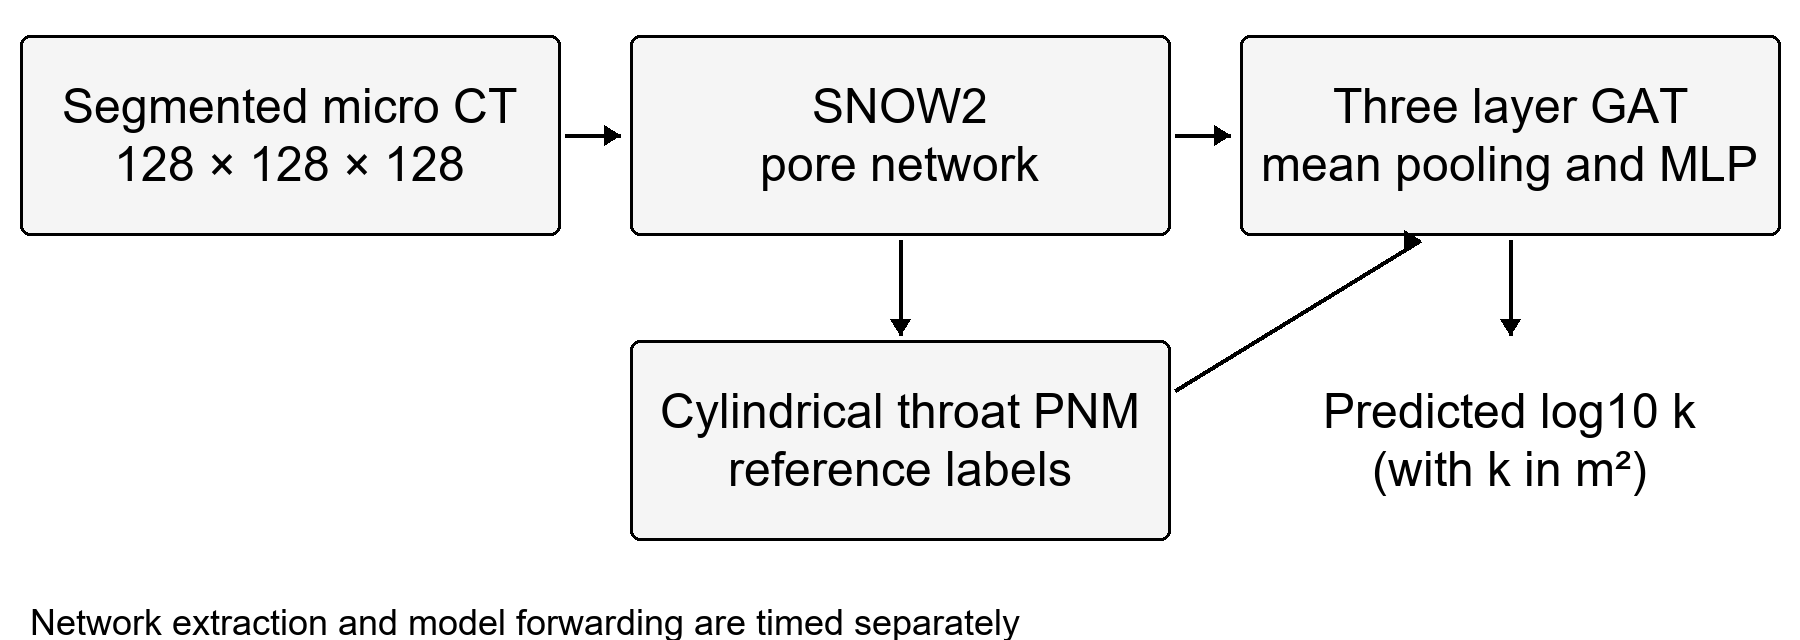
\includegraphics[width=.84\linewidth]{figure-1.png}
\caption{TopoFlow workflow. The PNM supplies training and evaluation targets separately from model inference.}
\label{fig:1}
\end{figure}
\subsection{Model Description}

The bulk model uses graph attention \cite{r15}. Its first layer has two 64-channel heads, giving 128 channels; the next two have one 64-channel head each. ELU and dropout follow each layer. Global mean pooling feeds a 64\ensuremath{\rightarrow}32\ensuremath{\rightarrow}1 MLP with ReLU and dropout. The original bulk encoder does not receive throat features.

The pooled GAT output is a scalar z used for standardized-target regression:
\[
z=\mathrm{MLP}\left( \frac{1}{\left| V\right|}\sum_{v\in V} {h}_{v}^{L}\right)
\]
Each attention layer updates a pore embedding by a weighted neighborhood sum:
\[
{h}_{v}^{l+1}=\mathrm{ELU}\left( \sum_{u\in N\left( v\right)\cup \left\{ v\right\}} {\alpha }_{vu}^{l}{W}^{l}{h}_{u}^{l}\right)
\]
\nopagebreak[4]
\[
{\alpha }_{vu}=\frac{\exp \left( {e}_{vu}\right)}{\sum_{j\in N\left( v\right)\cup \left\{ v\right\}} \exp \left( {e}_{vj}\right)}
\]
The coefficients \ensuremath{\alpha} are softmax-normalized over the neighbors and self-loop of pore v. Scores use a learned vector applied to concatenated transformed endpoint embeddings followed by LeakyReLU \cite{r15}. The two first-layer heads are concatenated. This local attention is distinct from the separately trained global throat-importance head used in the restriction experiment.

For the scale-normalized variant, d\textsubscript{0} is the geometric-mean diameter of physical pores. Inputs become \ensuremath{\log_{10}}(d/d\textsubscript{0}) and \ensuremath{\log_{10}}(V/d\textsubscript{0}\ensuremath{^{3}}); twice \ensuremath{\log_{10}}d\textsubscript{0} is subtracted from the target. Training-only means and standard deviations normalize features and targets. The geometry branch uses a 10\ensuremath{\rightarrow}16\ensuremath{\rightarrow}1 MLP with scalar output \ensuremath{z_g}. Prediction reconstructs the log target using the development residual mean \ensuremath{\mu}\textsubscript{t} and standard deviation \ensuremath{\sigma}\textsubscript{t}:
\[
\hat{y} =2{\log }_{10}{d}_{0}+{\mu }_{t}+{\sigma }_{t}\left( z+{z}_{g}\right)
\]
\begin{table}[!htbp]
\caption{Geometry used by the bulk and restriction models}
\label{tab:2}
\centering\small
\setlength{\tabcolsep}{4pt}
\renewcommand{\arraystretch}{1.18}
\begin{tabularx}{\linewidth}{@{}>{\RaggedRight\arraybackslash}p{.25\linewidth}>{\RaggedRight\arraybackslash}p{.31\linewidth}>{\RaggedRight\arraybackslash}X@{}}
\toprule
\textbf{Feature group} & \textbf{Bulk GAT} & \textbf{Restriction GAT} \\
\midrule
Pore geometry & Log diameter and volume & Normalized diameter and volume \\
Position and boundary & Not used & 3 coordinates and 2 boundary flags \\
Throat geometry & Not used & Log diameter, length and d\ensuremath{^{4}}/L proxy \\
Throat direction & Not used & 3 absolute direction components \\
Global features & 10 descriptors in ablation & Global edge-score normalization \\
\bottomrule
\end{tabularx}
\end{table}
\subsection{Mathematical Details}

The hydraulic reference assumes steady, incompressible creeping flow. Cylindrical throat conductance is g = \ensuremath{\pi}d\ensuremath{^{4}}/(128\ensuremath{\mu}L), using inscribed diameter d, direct pore-center distance L and viscosity \ensuremath{\mu} = 0.001 Pa\ensuremath{\cdot}s. Inlet and outlet pressures are 1 and 0 Pa. Nonspanning components are excluded and conservation residuals checked.

A conventional creeping-flow criterion is
\[
\mathrm{Re}=\frac{\rho v{D}_{h}}{\mu }<1
\]
where \ensuremath{\rho} is density, v is characteristic velocity and D\textsubscript{h} is hydraulic diameter. This criterion states the assumed flow regime; it is not a measured Reynolds number for every image. Effective permeability is obtained from the steady network flux through Darcy's relation:
\[
k=\frac{Q\mu L}{A\Delta P}
\]
Here Q is total volumetric flow rate, L is the physical image length in the flow direction, A is the original image cross-sectional area and \ensuremath{\Delta}P is the applied pressure difference. Artificial boundary conduits are included in the declared reference. The labels are PNM approximations, not LBM or measured ground truth \cite{r2}.

Training uses mean squared error in y = \ensuremath{\log_{10}}(k/m\ensuremath{^{2}}), or its training-standardized residual in the scale-normalized model:
\[
\mathrm{MSE}=\frac{1}{N}\sum_{i=1}^{N} {\left( {y}_{i}-{\hat{y} }_{i}\right)}^{2}
\]
Predictive R\ensuremath{^{2}} is calculated in log space using the mean reference value of the evaluated set:
\[
{R}^{2}=1-\frac{\sum_{i=1}^{N} {\left( {y}_{i}-{\hat{y} }_{i}\right)}^{2}}{\sum_{i=1}^{N} {\left( {y}_{i}-\bar{y} \right)}^{2}}
\]
Here N is the number of evaluated crops, y\textsubscript{i} is reference log permeability and \ensuremath{\hat{y}}\textsubscript{i} is its prediction. RMSE, MAE and R\ensuremath{^{2}} are recomputed from saved predictions. Negative test R\ensuremath{^{2}} is retained. Parent-balanced RMSE and pooled crop metrics are distinguished; seed variability is not treated as independent geological replication.

\subsection{Working Steps}

1) Input and separation: The development set contains 24 natural crops from Berea (8), C1 (7), C2 (6) and Estaillades (3). Outer validation holds out one complete parent scan, with inner selection on the other three. No crop from an outer test parent is used for feature scaling, target scaling or model selection.

2) Locked external test: After development selection, models are trained on all 24 development crops and tested on 32 crops, eight each from S1, S3, S5 and S9. Their voxel sizes are 8.683, 9.100, 3.997 and 3.398 \ensuremath{\mu}m. The primary GAT variant and its settings are fixed before inspecting these outcomes.

3) Feature assignment: The ten raw descriptors are porosity; the mean and population standard deviation of \ensuremath{\log_{10}} diameter and \ensuremath{\log_{10}} volume; \ensuremath{\log_{10}} pore and directed-edge counts; mean and population standard deviation of degree; and pore-radius CV. Each physical throat contributes two directed edges. GAT and physics ridge replace porosity by \ensuremath{\log_{10}}\ensuremath{\Phi} and \ensuremath{\log_{10}}(1\ensuremath{-}\ensuremath{\Phi}), omit mean log diameter, and subtract 3 \ensuremath{\log_{10}}d\textsubscript{0} from mean log volume, retaining ten inputs. ExtraTrees uses the raw vector. Ablations separately enable node/target scale normalization and this descriptor branch.

4) Training: The neural benchmark uses seeds 11, 22, 33, 44 and 55. The locked primary GAT uses learning rate 0.003, dropout 0.1, weight decay 0.001 and 14 epochs selected on development scans. GAT and GraphSAGE receive matching data and selection procedures. The graph-wise loss pairs one scalar target with one prediction per graph.

5) Restriction extension: A separate edge-aware model trains on eight development crops, two per parent. Seven node features add normalized coordinates and inlet/outlet flags; six edge features encode normalized diameter, length, a d\ensuremath{^{4}}/L proxy and absolute direction components. Three 32-channel GAT layers feed a symmetric 70\ensuremath{\rightarrow}32\ensuremath{\rightarrow}2 edge head. A global softmax predicts importance s, and a sigmoid gives leverage \ensuremath{\ell} bounded by 1\ensuremath{-}s. For diameter reduction q, the conductance multiplier is r=(1\ensuremath{-}q)\ensuremath{^{4}}. Changing one conductance gives a rank-one update of the linear network equations. The Sherman--Morrison identity \cite{r16} yields the loss expression below when s and \ensuremath{\ell} are the exact dissipation fraction and edge leverage. The GAT substitutes learned estimates; their accuracy determines response calibration. A derivation accompanies the source implementation:
\[
\mathrm{loss}=\frac{\left( 1-r\right)s}{1-\left( 1-r\right)\ell }
\]
\section{Results and Discussion}

\subsection{Permeability Prediction}

The evaluation uses natural-rock crops with parent-scan separation. Synthetic development examples and historical demonstration outputs are excluded from the reported benchmark. The hydraulic target is the same cylindrical-throat PNM for all compared bulk predictors.

Nested validation gives parent-balanced log-RMSE 0.8311 \ensuremath{\pm} 0.0200 for the normalized GAT with descriptors and 0.8713 \ensuremath{\pm} 0.0781 for matched GraphSAGE. Calibrated porosity KC gives 0.7525. The GAT improvement over GraphSAGE is modest and does not establish architectural superiority on four source groups.

The controlled GAT ablation yields parent-balanced log-RMSE 1.5528 for standard inputs, 0.9504 with normalization alone, 0.8933 with descriptors alone and 0.8311 with both. Thus, both additions help in development validation. This comparison separates feature and scale choices from an attention-specific explanation.

On the locked external test, the primary normalized GAT with descriptors gives log-RMSE 0.5687 \ensuremath{\pm} 0.0805 and log-R\ensuremath{^{2}} \ensuremath{-}0.7671. Physics ridge gives 0.2534 and 0.6547, respectively. The two single-addition GAT ablations obtain RMSE 0.4111 and 0.4131, but they are not retrospectively substituted for the primary model. Table 3 includes the fixed comparison.

Figure 2 summarizes external errors. Values for neural models are means over five independently trained seeds; the error bars show seed standard deviation. The simpler ridge and scaled-KC controls demonstrate that low-dimensional geometric information explains substantial variation in the reference labels. An accurate node-only predictor is therefore not, by itself, evidence that attention has learned the governing flow paths.

\begin{figure}[!htbp]
\centering
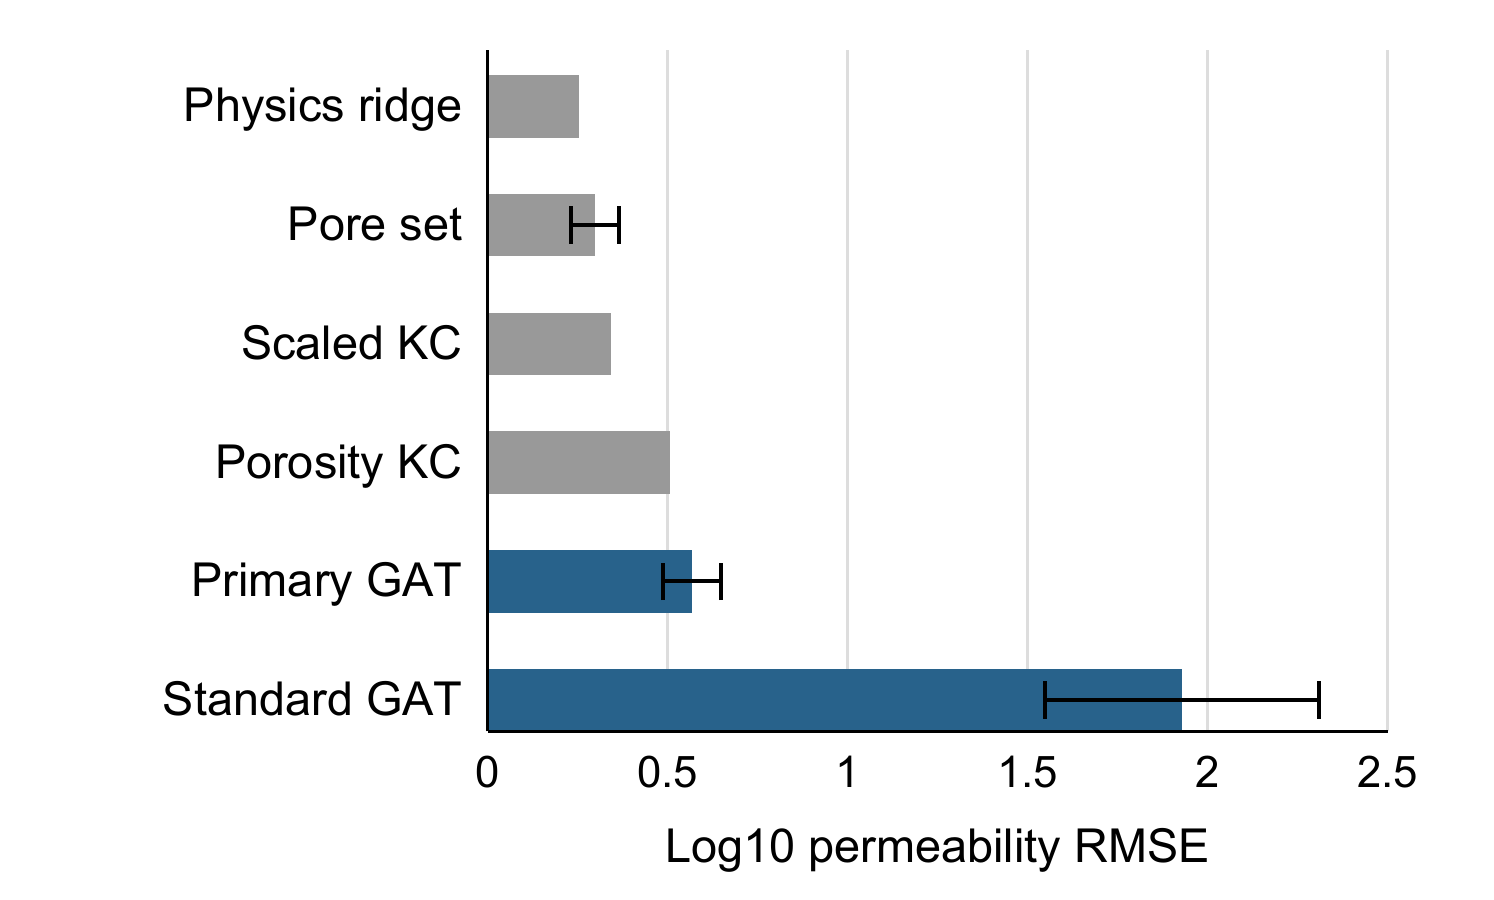
\includegraphics[width=.84\linewidth]{figure-2.png}
\caption{Locked external permeability comparison. Error bars show five-seed standard deviation; the fitted non-neural controls are deterministic.}
\label{fig:2}
\end{figure}
\subsection{Computational Cost}

Serial CPU measurements use one Torch/BLAS thread. Bulk-model forward timing uses ten warmups and thirty calls per crop, excluding file loading and feature normalization. Median GAT forward time is 1.72 ms across 24 crops. Separate measurements on one crop per development parent give median SNOW2 extraction 4.06 s and PNM solve 1.85 ms. These samples and operation scopes differ; their ratio is not an end-to-end speedup.

\begin{figure}[!htbp]
\centering
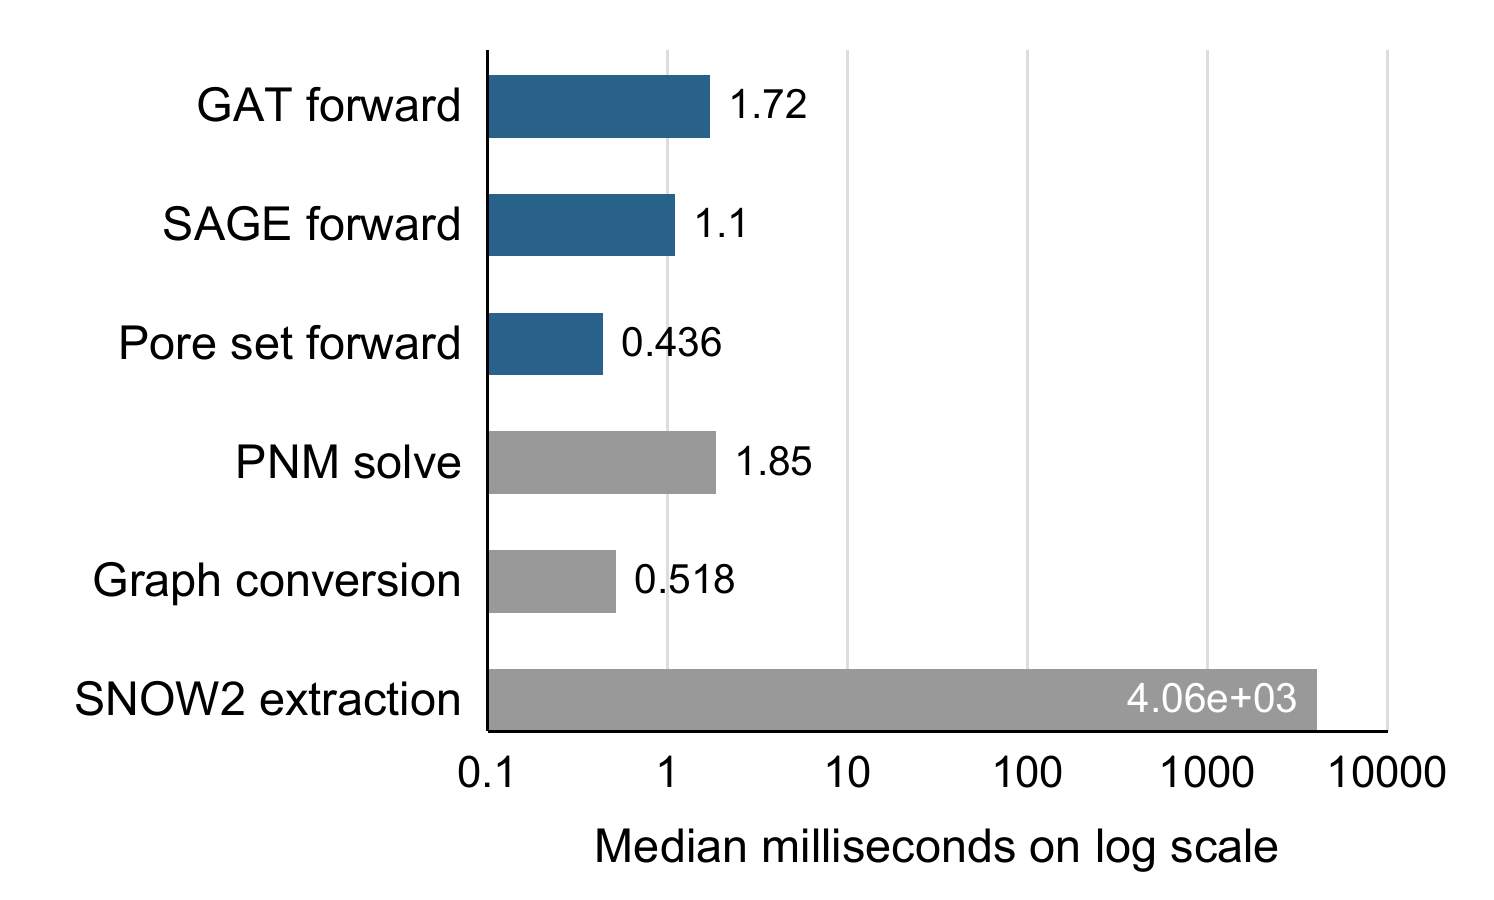
\includegraphics[width=.84\linewidth]{figure-3.png}
\caption{Measured component costs in the development benchmark. Extraction is measured on four crops and neural forwarding on 24; file loading and model loading are excluded.}
\label{fig:3}
\end{figure}
\begin{table}[!htbp]
\caption{Locked external permeability results on 32 crops}
\label{tab:3}
\centering\small
\setlength{\tabcolsep}{4pt}
\renewcommand{\arraystretch}{1.18}
\begin{tabularx}{\linewidth}{@{}>{\RaggedRight\arraybackslash}p{.30\linewidth}>{\centering\arraybackslash}X>{\centering\arraybackslash}p{.16\linewidth}>{\centering\arraybackslash}p{.16\linewidth}@{}}
\toprule
\textbf{Model} & \textbf{Log RMSE} & \textbf{Log R\ensuremath{^{2}}} & \textbf{Within \ensuremath{\times}2} \\
\midrule
Physics ridge & 0.253 & 0.655 & 75.0\% \\
Pore set + geometry & 0.298 \ensuremath{\pm} 0.066 & 0.503 & 66.9\% \\
Scaled KC & 0.343 & 0.368 & 53.1\% \\
GAT descriptors & 0.411 \ensuremath{\pm} 0.126 & 0.023 & 51.2\% \\
GAT normalized & 0.413 \ensuremath{\pm} 0.106 & 0.034 & 51.2\% \\
Porosity KC & 0.506 & -0.377 & 40.6\% \\
Primary GAT & 0.569 \ensuremath{\pm} 0.080 & -0.767 & 36.9\% \\
Standard GAT & 1.929 \ensuremath{\pm} 0.381 & -19.641 & 7.5\% \\
\bottomrule
\end{tabularx}
\end{table}
\subsection{Critical Throat Evaluation}

Partial throat narrowing leaves the original node-only GAT inputs unchanged, so that model returns exactly the same permeability. The edge-aware extension addresses this representation limitation. Guided GAT, guided mean GNN and guided edge MLP share importance supervision with weight 0.05; an unguided GAT is retained as a control. AdamW uses learning rate 0.003, weight decay 0.0001 and batch size two. Development-parent validation selects 15, 12, 22 and seven epochs, respectively; 20 checkpoints (four models \ensuremath{\times} five seeds) are frozen before the new scans are extracted.

The test uses S2, S4, S6, S7 and S8, with two opposite-corner 128\ensuremath{^{3}} crops per scan and voxel sizes 4.956, 8.960, 5.100, 4.803 and 4.892 \ensuremath{\mu}m. Eligible throats join physical pores in a topology-spanning component. Each method selects its own three highest and lowest scores plus three shared random throats. Selections are saved and hashed before hydraulic outcomes are calculated. Each throat is restricted individually at 10\%, 25\% and 50\%; the experiment is not simultaneous multi-throat clogging.

\begin{figure}[!htbp]
\centering
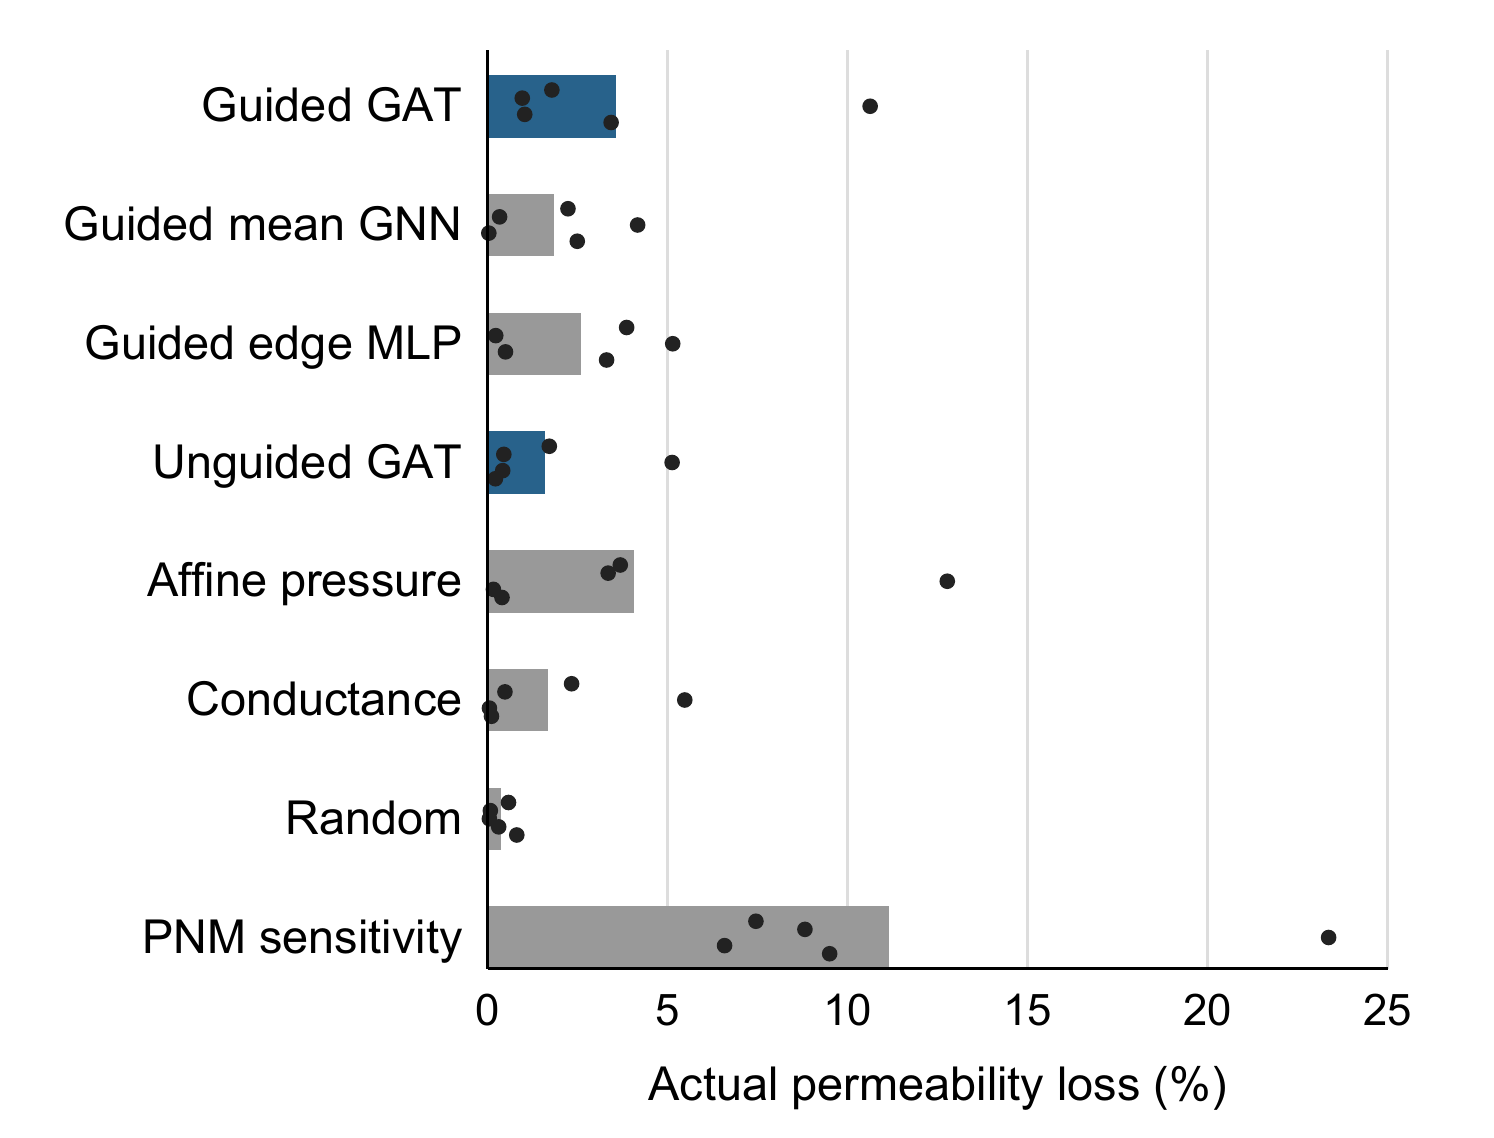
\includegraphics[width=.84\linewidth]{figure-4.png}
\caption{Actual loss from individual 50\% restrictions of top-selected throats. Bars show scan-balanced means; dots show the five scan means. PNM sensitivity requires a solved flow.}
\label{fig:4}
\end{figure}
Averaging first within crop and then equally across scans, guided-GAT top selections cause 3.57\% mean permeability loss, versus 0.37\% for random, 4.08\% for affine pressure, 2.61\% for guided MLP and 1.85\% for guided mean GNN. GAT versus affine pressure gives exact paired sign-flip p=0.625. With five scan groups the minimum two-sided p-value is 0.0625; seed counts and intervention counts do not increase the number of independent groups.

On the shared union of geometry-selected throats and three doses, 897 unique interventions yield guided-GAT response MAE 2.04 percentage points (pp), compared with 0.46 for no response, 0.75 for affine pressure and 1.92 for guided MLP. Although 78.3\% of interventions cause less than 0.1 pp loss, guided GAT also underperforms for losses of at least 1 pp: MAE 6.66 versus 4.51 for no response. Ranking information therefore coexists with poor amplitude calibration. No correction is fitted on these test outcomes.

Fresh sparse solves check 966 selected throat-dose interventions. Subsequent diagnostics reuse the same five scan groups and are explicitly post hoc. Shortest-path tortuosity has Spearman correlation 0.60 with GAT-minus-affine ranking advantage; coefficients for axial alignment, degree CV and cut density are 0.30, \ensuremath{-}0.50 and \ensuremath{-}0.30. These small-sample associations do not establish a validated topological threshold.

\subsection{Reference and Timing Limits}

Sixteen independently assembled, identical-conductance OpenPNM checks agree with the sparse reference to a maximum relative permeability difference of 2.1\ensuremath{\times}10\ensuremath{^{-14}}. This verifies numerical implementation. On supplied original S1/S5 maximal-ball networks, a Valvatne--Blunt shape-factor closure \cite{r17} differs from published network permeability by 12.5\% and 33.5\%. Closure, reservoir-boundary treatment and flow-axis differences remain material.

Full-volume SNOW calculations give 342.49 and 1187.48 mD for S1 and S5, versus published image Kz values 1312 and 4440 mD. The original-network checks do not reconcile that gap. PNM target uncertainty is therefore distinct from learning error, and the restriction results remain conditional on cylindrical inscribed-diameter throats. Location-dependent clogging has prior pore-scale treatments \cite{r18}; these fixed-network interventions do not simulate evolving deposits.

In the frozen restriction benchmark, one-thread warm CPU times average scan-wise median calls after five warmups and thirty repetitions. Guided GAT takes 5.31 ms per seed or 25.69 ms for a five-seed all-throat, three-dose ensemble. A base PNM solve takes 2.60 ms; three fresh 50\% solves take 7.81 ms excluding the base solve. Exact all-throat precomputation takes 13.67 ms and its cached response readout 0.058 ms. SNOW2 extraction averages 6.76 s per crop. The operation scopes differ and establish no GAT speed advantage. Each restriction GAT stores 22,280 parameter bytes. Observed process RSS is 371--387 MB with all twenty models resident; this is neither peak nor incremental model memory.

Named scans are the grouping units; they are not independently certified geological specimens. Four development parents, four bulk external parents and five restriction-test parents do not establish population-wide generalization. All diagnostics, numerical tests, fixed checkpoints and prediction tables are provided with the implementation at github.com/ShaunakRane914/Flow.

\section{Future Scope}

Independent voxel-resolved flow or measured permeability is needed to assess physical accuracy beyond the present PNM reference. This validation should use specimens from sources excluded from model development.

Further work should test segmentation and extraction settings, voxel resolution and conductance closures under a fixed evaluation protocol. Broader source coverage is also needed to test the exploratory topology associations and evaluate response calibration or a geometry-based model selector on fresh scans.

\section{Conclusion}

TopoFlow combines SNOW2 pore networks with graph attention for PNM permeability regression. Scale normalization and graph descriptors improved development performance, but physics ridge remained stronger on the locked external test: log-RMSE was 0.253, compared with 0.569 for the primary GAT.

The throat-aware GAT identified more consequential restrictions than random selection, while affine-pressure ranking gave the larger aggregate loss. Its response predictions overestimated the reference PNM losses. These findings show that useful throat ranking does not ensure accurate response calibration.

\paragraph*{Disclosure of Interests.} The authors have no competing interests to declare.

\begin{thebibliography}{99}
\bibitem{r1} Dong, H., Blunt, M.J.: Pore-network extraction from micro-computerized-tomography images. Physical Review E 80, 036307 (2009). \url{https://doi.org/10.1103/PhysRevE.80.036307}
\bibitem{r2} Gostick, J., et al.: OpenPNM: A pore network modeling package. Computing in Science \& Engineering 18(4), 60--74 (2016). \url{https://doi.org/10.1109/MCSE.2016.49}
\bibitem{r3} Wu, J., Yin, X., Xiao, H.: Seeing permeability from images: Fast prediction with convolutional neural networks. Science Bulletin 63(18), 1215--1222 (2018). \url{https://doi.org/10.1016/j.scib.2018.08.006}
\bibitem{r4} Hamilton, W.L., Ying, R., Leskovec, J.: Inductive representation learning on large graphs. Advances in Neural Information Processing Systems 30 (2017). arXiv:1706.02216
\bibitem{r5} Chapuis, R.P., Aubertin, M.: On the use of the Kozeny--Carman equation to predict the hydraulic conductivity of soils. Canadian Geotechnical Journal 40(3), 616--628 (2003). \url{https://doi.org/10.1139/t03-013}
\bibitem{r6} Qian, Y.H., d'Humières, D., Lallemand, P.: Lattice BGK models for Navier--Stokes equation. Europhysics Letters 17(6), 479--484 (1992). \url{https://doi.org/10.1209/0295-5075/17/6/001}
\bibitem{r7} Savalkar, V.A., Saini, G.S., Pawar, S.D.: Density-Aware Explainable Hybrid CNN--Transformer Framework for Automated BI-RADS Breast Density Classification in Mammographic Images. Journal of Intelligent Decision Making and Information Science 3(1s), 1003--1027 (2026). \url{https://doi.org/10.59543/jidmis.v3.480}
\bibitem{r8} Alzahrani, M.K., Shapoval, A., Chen, Z., et al.: Pore-GNN: A graph neural network-based framework for predicting flow properties of porous media from micro-CT images. Advances in Geo-Energy Research 10(1), 39--55 (2023). \url{https://doi.org/10.46690/ager.2023.10.05}
\bibitem{r9} Zhao, X., Zhong, Y., Li, P.: RTG-GNN: A novel rock topology-guided approach for permeability prediction using graph neural networks. Geoenergy Science and Engineering 243, 213358 (2024). \url{https://doi.org/10.1016/j.geoen.2024.213358}
\bibitem{r10} I'Anson, J.M., Simmons, M.J.H., Stitt, E.H., Gallen, R.W.: Using graph neural networks to predict the permeability of porous media. InterPore Journal 2(3) (2025). \url{https://doi.org/10.69631/ipj.v2i3nr47}
\bibitem{r11} Zhao, Q., Xiao, H.: An end-to-end differentiable, graph neural network-embedded pore network model for permeability prediction. Journal of Hydrology 675, 135602 (2026). \url{https://doi.org/10.1016/j.jhydrol.2026.135602}
\bibitem{r12} Imperial College London, Pore-scale Modelling Group: ImagesICPSC2007. Binary images and source headers. \url{https://imperialcollegelondon.box.com/v/ImagesICPSC2007}, last accessed 2026/10/22
\bibitem{r13} Imperial College London: Estaillades 1000\ensuremath{^{3}} micro-CT image, 3.31136 \ensuremath{\mu}m. Official archive: \url{https://imperialcollegelondon.box.com/shared/static/2n4lb95amz7fstk19q826uzu922eb4b1.zip}, last accessed 2026/10/22
\bibitem{r14} Gostick, J.T.: Versatile and efficient pore network extraction method using marker-based watershed segmentation. Physical Review E 96, 023307 (2017). \url{https://doi.org/10.1103/PhysRevE.96.023307}
\bibitem{r15} Veličković, P., et al.: Graph Attention Networks. International Conference on Learning Representations (2018). arXiv:1710.10903
\bibitem{r16} Sherman, J., Morrison, W.J.: Adjustment of an inverse matrix corresponding to a change in one element of a given matrix. The Annals of Mathematical Statistics 21(1), 124--127 (1950). \url{https://doi.org/10.1214/aoms/1177729893}
\bibitem{r17} OpenPNM: Valvatne--Blunt hydraulic conductance. Official implementation documentation, installed version 3.6.0. \url{https://openpnm.org/_modules/openpnm/models/physics/hydraulic_conductance/_funcs.html#valvatne_blunt}, last accessed 2026/10/22
\bibitem{r18} Nassiri, S., van Paassen, L., Mahabadi, N.: Evolution of porous media and porosity--permeability relations during biogeochemical clogging processes: A pore-scale simulation study. Computers and Geotechnics 198, 108292 (2026). \url{https://doi.org/10.1016/j.compgeo.2026.108292}
\end{thebibliography}
\end{document}
